
\chapter{Einleitung}
\label{ch: Einleitung}
	

		Das Thema der künstlichen Intelligenz (KI) dringt zunehmend in den Alltag des Menschen ein. In den Jahren 2017 und 2018 wurden insgesamt über 100 Millionen \textit{Smart Home} Geräte wie \textit{Amazons Alexa} oder der \textit{Google Assistant} verkauft \cite{smart}. Derartige Technologien begleiten den Menschen jedoch nicht nur im Alltag, sondern auch in der Transport- und Logistikbranche.\\
		
		Eine Potenzialanalyse zur künstlichen Intelligenz der Firma \textit{Sopra Steria} zeigt, dass bereits im Jahr 2017 20 \% aller befragten Unternehmen derartige Systeme einsetzten \cite{sopra}. Den zukünftigen Einsatz in ihrer Logistik planten 37 \% \cite{sopra}. Die Implementierung solcher Systeme hat Einfluss auf verschiedene Eigenschaften der Wertschöpfungskette \cite{sopra}. Ein Beispiel für ein derartiges System ist das autonome Logistikfahrzeug (ALF), das in Abbildung \ref{fig: Darstellung des ALFs} zu sehen ist.
		
		\begin{figure}[H]
			\begin{minipage}[b]{0.49\textwidth}
				(a)
				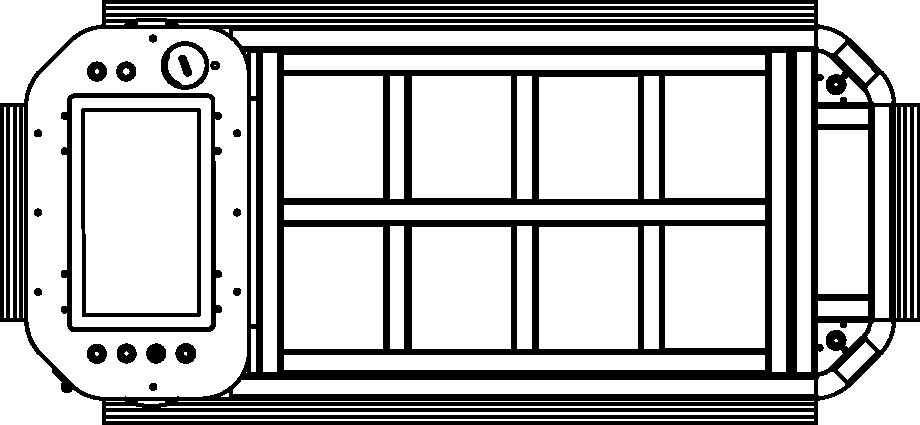
\includegraphics[width=0.9\textwidth]{Bilder/oben.pdf}
			\end{minipage}
			\begin{minipage}[b]{0.49\textwidth}
				(b)
				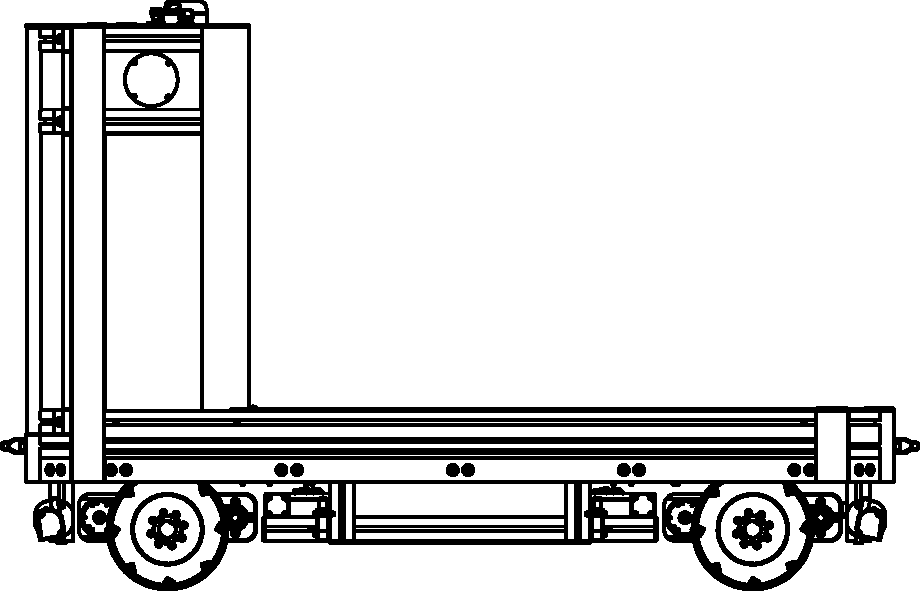
\includegraphics[width=0.9\textwidth]{Bilder/seite.pdf}
			\end{minipage}
			\centering
			\caption{(a) Darstellung des ALFs aus der Draufsicht. (b) Abbildung des ALFs aus der Seitenansicht.}
			\label{fig: Darstellung des ALFs}
		\end{figure}
		
		Die Idee hinter dem ALF ist es, ein Fahrzeug zu entwickeln, das nach Fertigstellung Logistikaufgaben am Standort der Hochschule Bochum löst. Es dient im Labor für Antriebstechnik der Hochschule Bochum als Versuchs- und Entwicklungsplattform für praktische Anwendungen \cite{Bachelorarbeit}. Der Entwicklungsprozess stellt sich aus der Bearbeitung diverser Bachelor- und Masterarbeiten zusammen, die sowohl Hardware- als auch Softwareintegrationen vorsehen \cite{Bachelorarbeit}.\\
		
		Bisher wurden zwei Abschlussarbeiten inklusive der praktischen Anwendung am ALF geschrieben \cite{alf, Bachelorarbeit}. Dennis Hotze und Dominik Eickmann entwickelten in ihrem Masterprojekt das Fahrzeug und konnten Fahraufgaben ferngesteuert und manuell erledigen \cite{alf}. Während der darauffolgenden Bachelorarbeit wurde eine Schlupfkompensation entwickelt, die den Drift am Fahrzeug durch Eingabe von Umgebungsinformationen verhindert \cite{Bachelorarbeit}. Weiterhin wurden Funktionen entwickelt, um grundlegende und autonome Fahraufgaben zu lösen \cite{Bachelorarbeit}.\\
		
		Der tägliche Kontakt zu Menschen ist nicht nur für die Anwendung des ALFs, sondern auch für andere Transportfahrzeuge im öffentlichen Raum charakteristisch. Kreuzen sich die Wege eines autonomen Fahrzeugs mit der einer oder mehrerer Personen, darf es in keiner Weise zur Kollision kommen. Das ALF zählt mit einem Maximalgewicht von 600 kg zu der Art von Fahrzeugen, die bei einem Zusammenstoß Verletzungen hervorrufen können. Ein solches System muss folglich in der Lage sein, bei einer Annäherung von Personen eine gesonderte Gefahreneinschätzung vorzunehmen.\\
				
		Ein weiteres, übliches Szenario solcher Systeme im öffentlichen Raum ist die Bedienung durch nicht autorisierte Personen. Für derartige Zwecke muss ein Mensch nicht nur als bewegtes Objekt, sondern auch als solcher erkannt werden. Das Hauptziel dieser Masterarbeit ist die Entwicklung einer Personenerkennung.\\
		
		Weiterhin wird das System nicht nur Personen detektieren, sondern diese auch wiedererkennen können. Dies bedeutet im praktischen Kontext, dass eine Person dem Roboter bekannt ist und bei einer Erkennung zugeordnet wird. Das Fahrzeug wird im Rahmen dieses Projekts auf die Erkennung von Personen beschränkt, da es im Einsatz an der Hochschule Bochum selten zu Begegnungen mit Tieren oder anderen Lebewesen kommt.\\
				
		Während der Bearbeitung von Transport- oder Fahraufgaben eines autonomen Fahrzeugs kann es zu diversen Komplikationen kommen. Beispielsweise können besonders im Anwendungsbereich der Hochschule Bochum Objekte den Verlauf einer Route unterbrechen und ein Ziel sogar unerreichbar machen. Häufig können diese Probleme durch menschliche Hilfe beseitigt werden, was wiederum eine Interaktion mit umstehenden Personen voraussetzt. Demnach wird in dieser Masterarbeit ein System zur Steuerung des ALFs mithilfe von Sprache entwickelt und am Fahrzeug implementiert.\\
		
		Eine Besonderheit dieser Masterarbeit ist die theoretische und praktische Entwicklung parallel zu einem weiteren Projekt. \textit{Hannes Dittmann} entwickelt in seiner Masterarbeit eine Sprachverarbeitung zur Klassifikation von Sprache \cite{Dittmann}. Diese stellt ein auditives \textit{Mensch-Maschine-Interface} (MMI) her. So kann eine Person über ein Aufnahmegerät mit dem System kommunizieren \cite{Dittmann}. Die oben genannte Steuerung wird mithilfe von Herrn \textit{Dittmanns} Sprachverarbeitung realisiert und zusammengeführt.\\
		
		Beide Masterarbeiten bilden im praktischen Kontext ein überarbeitetes Gesamtsystem des bereits bestehenden autonomen Logistikfahrzeugs \cite{Dittmann}. Die genannten Ziele sind im angehängten Lastenheft \ref{it: Lastenheft} festgehalten. Die erarbeiteten Ergebnisse werden so anhand eines Verifikationsplans am Fahrzeug geprüft.\\
		
		Die Struktur dieser Masterthesis ist in 4 Kapiteln gegliedert. Beginnend mit Kapitel \ref{ch: Grundlagen} werden die Grundlagen der eingesetzten Methoden und Systeme vermittelt. Hierbei werden Grundbegriffe des Themenbereichs der künstlichen Intelligenz und insbesondere der neuronalen Netze erklärt. Kapitel \ref{ch: Konzeptionierung} zeigt, wie die vermittelten Grundlagen zu einem System zusammengeführt und verwendet werden. Eine Evaluierung der im Feld getesteten Personenerkennung ist in Kapitel \ref{ch: Verifikation} beschrieben. Ein Vergleich alternativer Lösungen ist dort ebenfalls präsentiert. Das letzte Kapitel beschreibt zusammenfassend die gesamte Masterarbeit und gibt einen Ausblick für zukünftige Projekte am ALF. \\
		
		
		
		
		
		
	